\documentclass[a4paper,10pt]{article}
\usepackage[utf8]{inputenc}
\usepackage[T1]{fontenc}
\usepackage[ngerman]{babel}
\usepackage[sfdefault]{roboto}
\usepackage{geometry}
\usepackage{enumitem}
\usepackage{titlesec}
\usepackage[hidelinks]{hyperref}
\usepackage{graphicx}
\usepackage{tabularx}
\usepackage{array}
\usepackage{sectsty}
\usepackage{xcolor}
\usepackage{csquotes}
\usepackage{fontawesome5}

\geometry{left=2.5cm,right=2.5cm,top=2.5cm,bottom=2.5cm}
\definecolor{sectionblue}{RGB}{38, 97, 150}
\definecolor{sectiongreen}{RGB}{48, 128, 90}
\definecolor{sectiongray}{RGB}{90, 90, 90}
\setlength{\parindent}{0pt}
\sectionfont{\color{sectionblue}\large\bfseries\underline}
\titleformat{\section}{\color{sectionblue}\large\bfseries}{}{0em}{\underline}

\begin{document}

\noindent
\begin{minipage}[c]{0.72\textwidth}
  {\LARGE\color{sectionblue}\textbf{Sascha Rose}}\\[0.5em]
  {\color{sectionblue}\textbf{Software Engineer}}\\[1.5em]
  \textcolor{sectionblue}{\faEnvelope}\hspace{0.5em}sascha.rose@gmail.com\\[0.25em]
  \textcolor{sectionblue}{\faPhone}\hspace{0.5em}+49 179 50 898 30\\[0.25em]
  \textcolor{sectionblue}{\faHome}\hspace{0.5em}53508 Mayschoß (Cologne / Bonn / Germany)\\[1em]
  \textcolor{sectionblue}{\faGithubSquare}\hspace{0.5em}\href{https://github.com/rsascha}{github.com/rsascha}\\[0.25em]
  \textcolor{sectionblue}{\faInfoCircle}\hspace{0.5em}\href{https://www.freelancermap.de/profil/senior-fullstack-developer-react-react-native-nodejs-javascript-typescript}{freelancermap.de/profil}\\[0.25em]
  \textcolor{sectionblue}{\faInfoCircle}\hspace{0.5em}\href{https://agentur.actyvyst.de/}{actyvyst.de}\\[1em]
  \textcolor{sectiongreen}{\faSeedling}\hspace{0.5em}Available as of June 2025\\
\end{minipage}
\hfill
\begin{minipage}[c]{0.25\textwidth}
  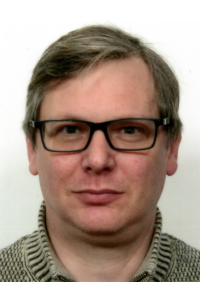
\includegraphics[width=\textwidth]{assets/sascha-rose.png}
\end{minipage}

% What I'm Looking For
\vspace{1.5em}
\section*{What I'm Looking For}
Seeking opportunities in web, app or backend development — either independently
or in cooperation with trusted colleagues from actyvyst GmbH.
Open to permanent positions.

% What I Bring to the Table
\vspace{1.5em}
\section*{What I Bring to the Table}
Full-stack developer with 20+ years of experience in software development,
architecture, and IT operations.
I specialize in modern web, app, server and cloud technologies — designing
scalable, robust, and maintainable systems.

\vspace{1em}

I’m experienced in quality assurance for long-term projects — covering unit,
integration and end-to-end testing. I also focus on security-related aspects
and their seamless automation and integration into daily development and CI/CD
pipelines.

\vspace{1em}

With a strong focus on continuous learning, and innovation, I stay up to date
with current tech trends and best practices.

\vspace{1em}

My experience working with interdisciplinary teams allows me to communicate
technical decisions effectively and lead implementations with confidence.

\vspace{1em}

I’m skilled at bridging the gap between developers and management — translating
technical challenges into business-relevant language and vice versa.

% Core Tech Stack
\vspace{1.5em}
\textbf{\textcolor{sectionblue}{Core Tech Stack:}}\\
React, HTML/CSS, React Native, Node.js (Express), TypeScript

% Languages
\vspace{1.5em}
\textbf{\textcolor{sectionblue}{Languages:}}\\
German (native), English (fluent)

% Where I Gained Experience
\section*{Where I Gained Experience}

% QiV
\vspace{1.5em}
\begin{tabularx}{\textwidth}{>{\raggedright}p{4.5cm}X}
  \textbf{\color{sectionblue}Software Engineer} \\
  {\color{sectiongray}2024–2025}                \\
  \vspace{1.5em}
  QiV – Qualit{\"a}t im Verkehr                 \\
  System for Recording Traffic Countings        \\
  {\color{sectiongray}actyvyst GmbH}
   &
  Mobile app for Android for recording and transmitting traffic countings.
  Traffic counters can use this app to record configurable interviews and
  count data. To ensure the use of the app even without a network, the data
  is recorded offline and then transmitted to the central server, where it is
  consolidated and validated in an evaluation system.
  \begin{center}
    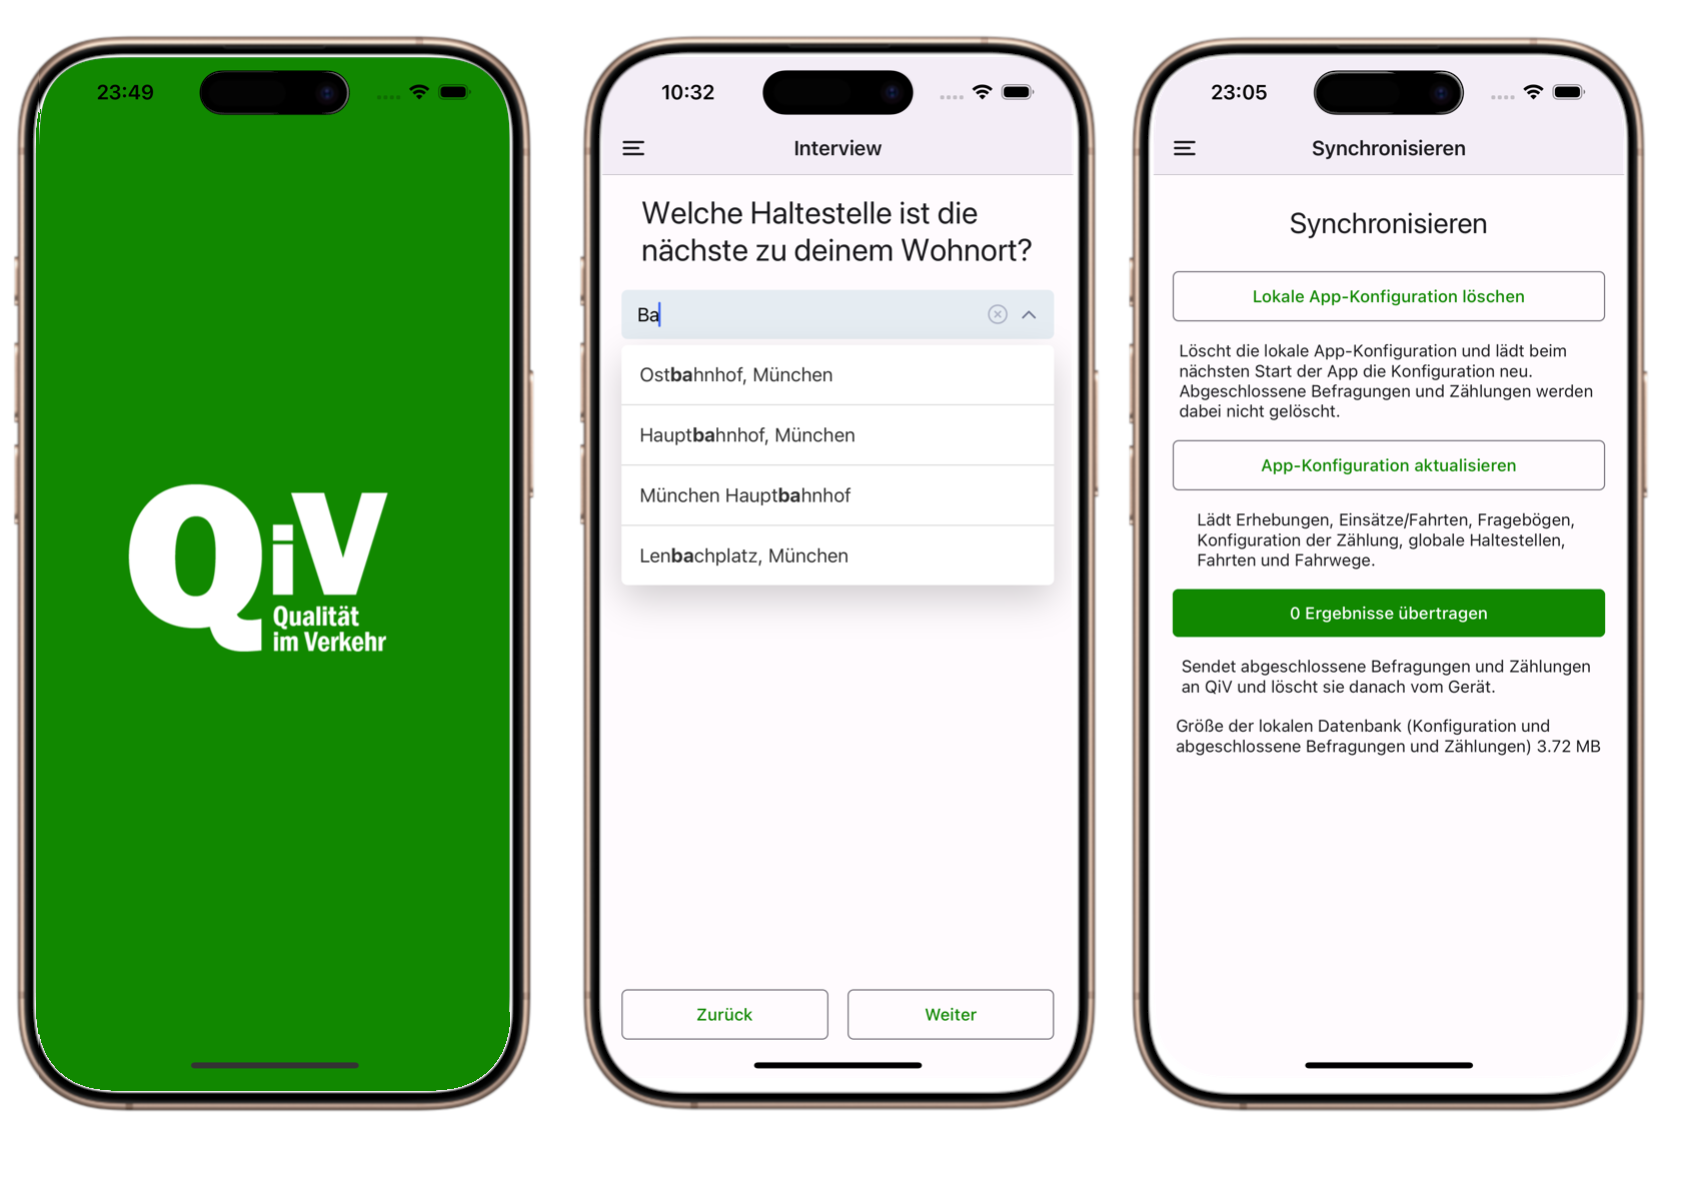
\includegraphics[width=0.8\linewidth]{assets/qiv.png}
  \end{center}
  \textbf{Technologies:} React, React Native, Node.js (Express), TypeScript,
  Excel: Power Query, AddIn (VB Script), TaskPane (React), .Net (C\#),
  postgres, GitHub Actions, Render.
\end{tabularx}

\vspace{1em}
\noindent{\color{sectionblue}\rule{\textwidth}{0.4pt}}
\vspace{1em}

% badenova
\begin{tabularx}{\textwidth}{>{\raggedright}p{4.5cm}X}
  \textbf{\color{sectionblue}Software Engineer}                                  \\
  {\color{sectiongray}2022–2025}                                                 \\
  \vspace{1.5em}

  Planning, implementation, maintenance, and further development of a mobile app
  for end customers of an energy provider.\@                                     \\ {\color{sectiongray}actyvyst
  GmbH} & The app enables meter reading (including camera integration), provides
  consumption forecasts, and supports monthly payment optimization. I developed
  the backend systems, integrated APIs, and set up the entire infrastructure.
  \begin{center}
    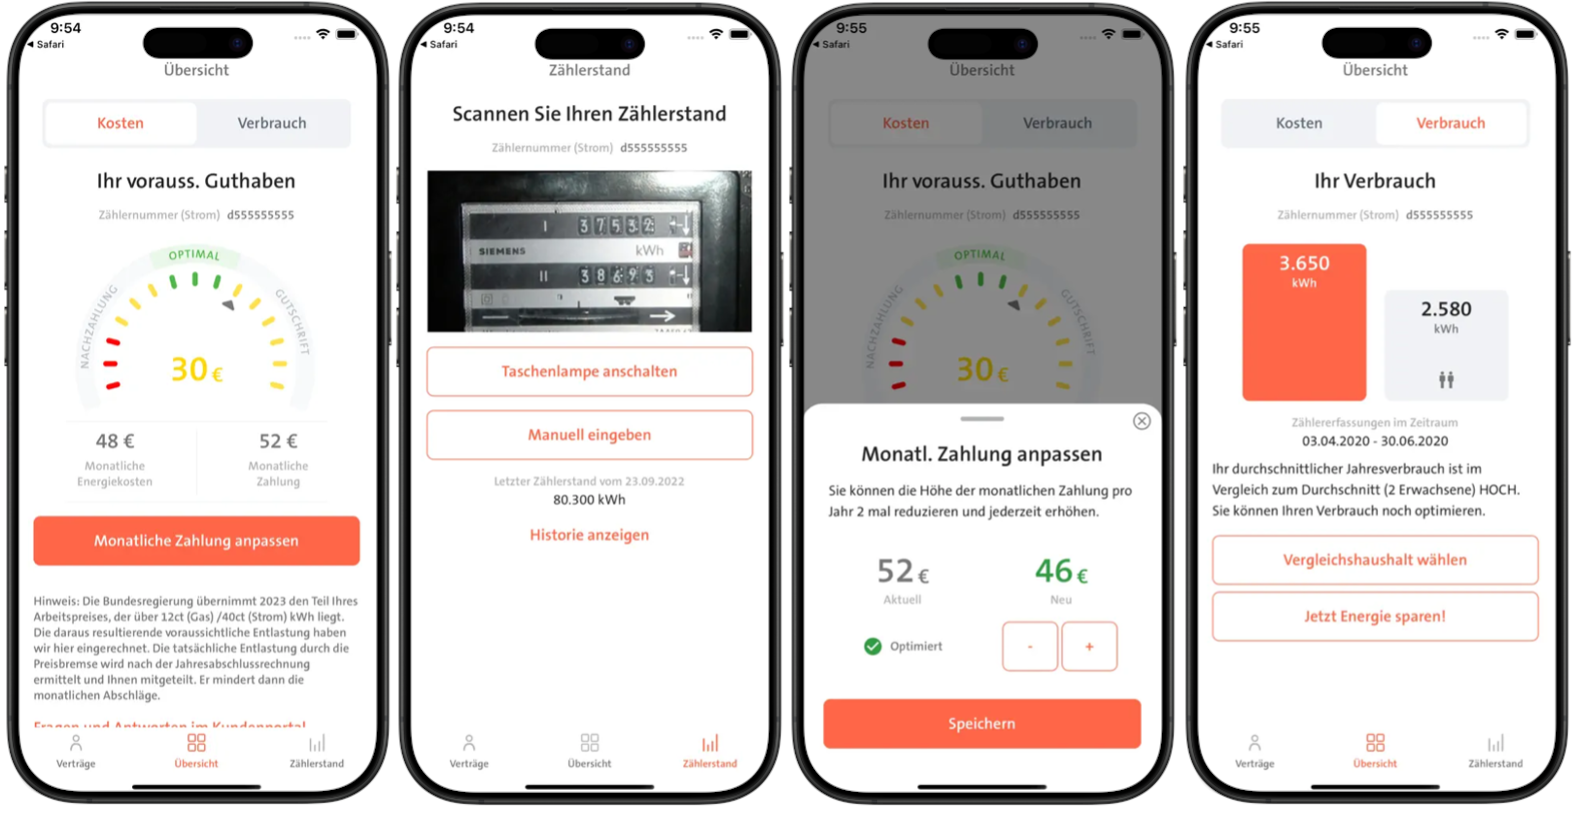
\includegraphics[width=0.8\linewidth]{assets/badenova.png}
  \end{center}
  \textbf{Technologies:} React, React Native, Node.js (NestJS, Express), Type-Script, Python (FastAPI), postgres, GitHub Actions, AWS, Kyma (SAP), Kubernetes.
\end{tabularx}

\vspace{1em}
\noindent{\color{sectionblue}\rule{\textwidth}{0.4pt}}
\vspace{1em}

% campus talents
\begin{tabularx}{\textwidth}{>{\raggedright}p{4.5cm}X}
  \textbf{\color{sectionblue}Lecturer} \\
  {\color{sectiongray}2023–2025}       \\
  \vspace{1.5em}
  Taktsoft Campus Talents              \\
  {\color{sectiongray}actyvyst GmbH}
   &
  I worked part-time as a lecturer, helping career changers enter the field of software development.
  \begin{center}
    
\includegraphics[width=0.8\linewidth]{assets/logo-campus-talents.png}
  \end{center}
  I taught technologies such as JavaScript, React, web development, app development with React Native (iOS, Android), and API development with Node.js and Express.
\end{tabularx}

\vspace{1em}
\noindent{\color{sectionblue}\rule{\textwidth}{0.4pt}}
\vspace{1em}

% Awareness Kitchen
\begin{tabularx}{\textwidth}{>{\raggedright}p{4.5cm}X}
  \textbf{\color{sectionblue}Software Engineer}                              \\
  {\color{sectiongray}2024}                                                  \\
  \vspace{1.5em}
  React Native development for the Düsseldorf-based agency Awareness Kitchen \\
  {\color{sectiongray}actyvyst GmbH}
   &
  Development of the Escape Box app, which acts as a game master for an escape room experience and is designed as an interactive learning game for security awareness training. The app coordinates the game as a “timekeeper” and provides multimedia support, including a timer function to solve the challenges.
  \begin{center}
    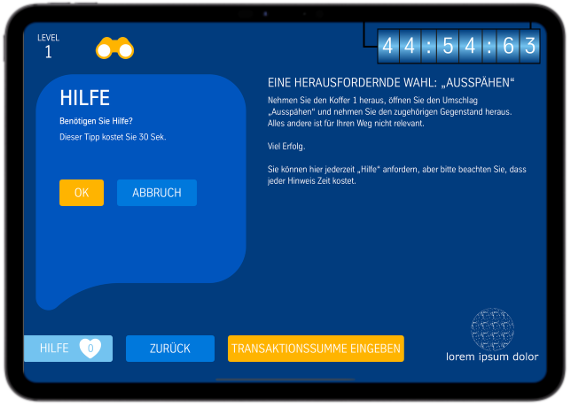
\includegraphics[width=0.8\linewidth]{assets/awareness-kitchen.png}
  \end{center}
  \textbf{Technologies:} Expo, React Native, Gesture Handling, Animations, Videos, deployed as an unlisted app in the App Store.
\end{tabularx}

\vspace{1em}
\noindent{\color{sectionblue}\rule{\textwidth}{0.4pt}}
\vspace{1em}

% actyvyst
\begin{tabularx}{\textwidth}{>{\raggedright}p{4.5cm}X}
  \textbf{\color{sectionblue}Software Engineer} \\
  {\color{sectiongray}2022–}                    \\
  \vspace{1.5em}
  actyvyst GmbH
   &
  I have been a shareholder and employee of actyvyst GmbH.
\end{tabularx}

\vspace{1em}
\noindent{\color{sectionblue}\rule{\textwidth}{0.4pt}}
\vspace{1em}

% freelance
\begin{tabularx}{\textwidth}{>{\raggedright}p{4.5cm}X}
  \textbf{\color{sectionblue}Software Engineer} \\
  {\color{sectiongray}2022}                     \\
  \vspace{1.5em}
  Freelancer
   &
  Freelance software projects under the umbrella of actyvyst GmbH.
\end{tabularx}

\vspace{1em}
\noindent{\color{sectionblue}\rule{\textwidth}{0.4pt}}
\vspace{1em}

% Amadeus Leisure IT GmbH - Aachen
\begin{tabularx}{\textwidth}{>{\raggedright}p{4.5cm}X}
  \textbf{\color{sectionblue}Software Engineer} \\
  {\color{sectiongray}2019–2021}                \\
  \vspace{1.5em}
  Senior Developer at Amadeus Leisure IT GmbH, Aachen
   &
  As a Senior Developer, I led software development in the field of internet booking engines for travel portals.
  My tasks included frontend and microservice development, as well as major contributions to infrastructure setup.
  I introduced trunk-based development, automated deployments, implemented CI/CD pipelines, standardized test automation (unit, E2E, and integration tests), and established quality and security gates to ensure software quality and security.

  \textbf{Technologies:} Angular, TypeScript, NodeJS (NestJS), OpenAPI, ORM, MongoDB,
  Redis, Keycloak, Kubernetes, Kustomize, NGINX, Prometheus, ELK, Jenkins,
  Docker, Artifactory, Confluence, Jira, Jest, Cypress, SonarQube, Fortify,
  BlackDuck, OWASP ZAP.\@
\end{tabularx}

\vspace{1em}
\noindent{\color{sectionblue}\rule{\textwidth}{0.4pt}}
\vspace{1em}

% Amadeus Leisure IT GmbH - Bonn
\begin{tabularx}{\textwidth}{>{\raggedright}p{4.5cm}X}
  \textbf{\color{sectionblue}Head of Software Development} \\
  {\color{sectiongray}2010–2019}                           \\
  \vspace{1.5em}
  Amadeus Leisure IT GmbH, Bonn
   &
  In this role, I managed up to 20 employees in software development at the Bonn location.
  I was also an IHK-certified trainer for IT specialists in application development.
  I led the transformation of the company into an agile organization and oversaw the migration of software solutions into the Amadeus Group.
  A key responsibility was leading travel agency solutions for the DACH market.
  From 2010 to 2014, I was also instrumental in developing and rolling out the “Trusted Reviews” platform internationally, providing verified hotel reviews from real travelers.
\end{tabularx}

\vspace{1em}
\noindent{\color{sectionblue}\rule{\textwidth}{0.4pt}}
\vspace{1em}

% pixell daten & design GmbH
\begin{tabularx}{\textwidth}{>{\raggedright}p{4.5cm}X}
  \textbf{\color{sectionblue}Team Lead in Software Development} \\
  {\color{sectiongray}2000–2010}                                \\
  \vspace{1.5em}
  pixell daten \& design GmbH, Bonn
   &
  In my first position, where I later became a partner, I was part of a start-up specializing in digitalizing marketing processes in the travel industry.
  We developed the live pricing solution \enquote{pixell Travel Suite} which was licensed by major companies such as Expedia, TUI, HRS, REWE, and RCCL.\@
  We also developed the first mobile app in Germany for booking package holidays,
  used by Expedia, TUI, and Kuoni. Our work was recognized with the Travel
  Technology Innovation Award and the Travel Industry Club Award.
\end{tabularx}

\vspace{1em}
\noindent{\color{sectionblue}\rule{\textwidth}{0.4pt}}
\vspace{1em}

% Uni
\begin{tabularx}{\textwidth}{>{\raggedright}p{4.5cm}X}
  \textbf{\color{sectionblue}Student} \\
  {\color{sectiongray}1995–2000}      \\
  \vspace{1.5em}
   &
  Studied Diplom-Informatik (Computer Science), University of Bonn
\end{tabularx}

\end{document}